\documentclass[12pt]{article}
\usepackage{graphicx,float}
\usepackage{listings}
\usepackage{xcolor}

\graphicspath{ {./fig/} }

\definecolor{codegreen}{rgb}{0,0.6,0}
\definecolor{codegray}{rgb}{0.5,0.5,0.5}
\definecolor{codepurple}{rgb}{0.58,0,0.82}
\definecolor{backcolour}{rgb}{0.95,0.95,0.92}


\lstdefinelanguage{SPICE}{
  keywords={tran,ac,dc,subckt,meas,plot,print,control,run,end,endc, hardcopy},
  morecomment=[l]{*},
  morecomment=[l]{\$},
  morecomment=[s]{/*}{*/},
  morestring=[b]',
  morestring=[b]",
  ndkeywords={r,r1,r2,r3,r4,r5,l,l1,l2,l3,l4,l5,c,c1,c2,c3,c4,c5,v,vin,m,m1,m2,m3,m4,m5,d,d1,d2,d3,d4,d5,vdb, pulse,sin,i,pwl,exp},
  keywordstyle=\color{blue}\bfseries,
  ndkeywordstyle=\color{codegreen}\bfseries,
  identifierstyle=\color{black},
  commentstyle=\color{purple}\ttfamily,
  stringstyle=\color{red}\ttfamily,
  sensitive=true
}
\lstdefinestyle{mystyle}{
	backgroundcolor=\color{backcolour},   
    commentstyle=\color{codegreen},
    keywordstyle=\color{magenta},
    numberstyle=\tiny\color{codegray},
    stringstyle=\color{codepurple},
    basicstyle=\ttfamily\footnotesize,
    breakatwhitespace=false,         
    breaklines=true,                 
    captionpos=b,                    
    keepspaces=true,                 
    numbers=left,                    
    numbersep=5pt,                  
    showspaces=false,                
    showstringspaces=false,
    showtabs=false,                  
    tabsize=4
}

\lstset{style=mystyle}


% Title[Enter title of the experiment here]
\title{EE230: Lab-7\\
Active Filters}

% Author[Enter details of author here]
\author{Prateek Garg, 20D070060}

% begin the document.
\begin{document}
\noindent
% make a title page.[this creates title page]
\maketitle

\section{Overview of the experiment} %[This segment creates Section as seen in document]

\subsection{Aim of the experiment}%[This segment creates sebsections under the same section]
The aim of the experiment is to create Active filter circuits using opamp LM741 and plot gain vs frequency.
g the values to a python script to plot them using Matplotlib.

\section{Design}
\subsection{Sallen-Key Active Low-Pass Filter}
\makebox[\textwidth]{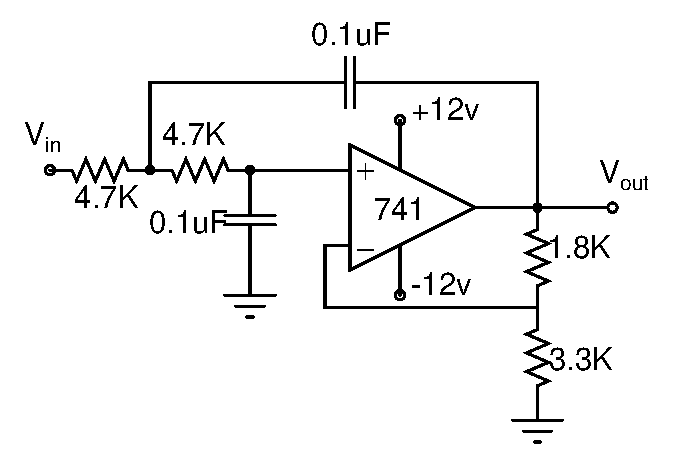
\includegraphics[width=\paperwidth]{lpf.eps}}
\subsection{Sallen-Key Active High-Pass Filter}
\makebox[\textwidth]{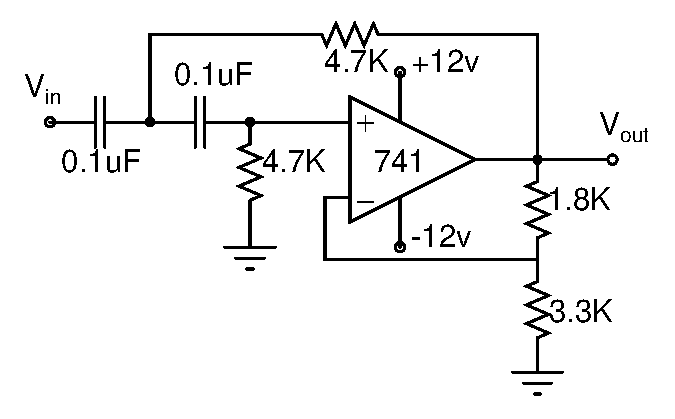
\includegraphics[width=\paperwidth]{hpf.eps}}
\subsection{Multiple-feedback Active Bandpass Filter}
\makebox[\textwidth]{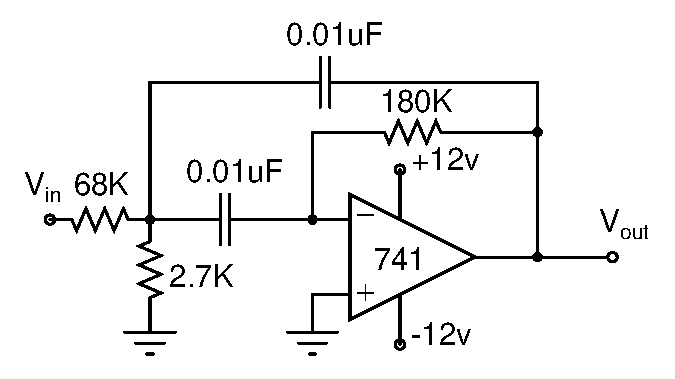
\includegraphics[width=\paperwidth]{Bpf.eps}}

\section{Experimental results}
\subsection{Sallen-Key Active Low-Pass Filter}
\makebox[\textwidth]{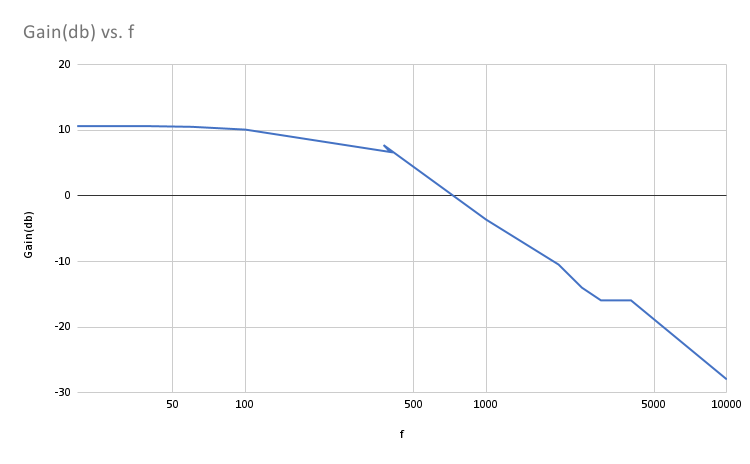
\includegraphics[width=\paperwidth]{LPF.png}}
Theoretical Cut-off frequency=338.62Hz
Experimental Cut-off frequency=375Hz
Roll-off=-22.6
Experimental Values quite match the theoretical Expectations.
\subsection{Sallen-Key Active High-Pass Filter}
\makebox[\textwidth]{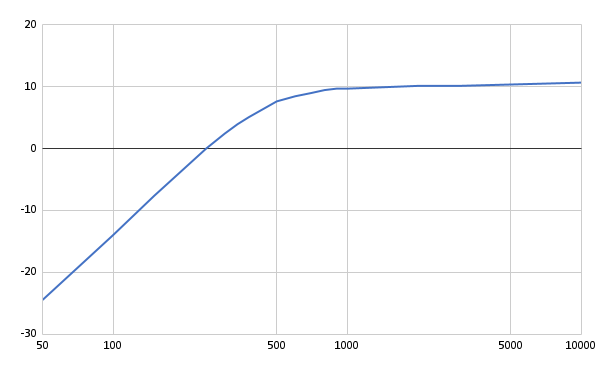
\includegraphics[width=\paperwidth]{Hpf.png}}
Theoretical Cut-off frequency=338.62Hz
Experimental Cut-off frequency=400Hz
Roll-off=36.124
Experimental Values quite match the theoretical Expectations.
\subsection{Multiple-feedback Active Bandpass Filter}
\makebox[\textwidth]{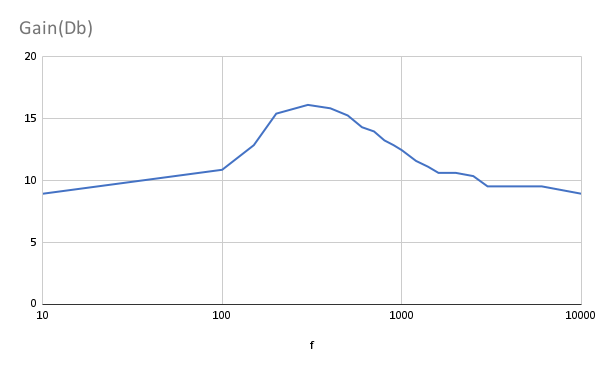
\includegraphics[width=\paperwidth]{Bpf.png}}

\section{Experiment completion status}
All the sections were completed
\end{document}
